\documentclass[12pt,notitlepage,]{article}
\usepackage[a4paper, top=0.7in, left=0.7in, right=0.7in, bottom=0.7in]{geometry}
\usepackage[utf8]{inputenc}
\usepackage[english]{babel}
\usepackage{hyperref}
\usepackage{xcolor}
\hypersetup{
    colorlinks,
    linkcolor={red!50!black},
    citecolor={blue!50!black},
    urlcolor={blue!80!black}
}
\usepackage{csquotes}
\usepackage{amsmath}
\usepackage{amssymb}
\usepackage{caption}
\usepackage{subcaption}
\captionsetup{width=0.8\textwidth,font+=it}

\usepackage{listings}
\lstset{captionpos=b, frame=lines, xleftmargin=1em, framextopmargin=0.5em, framexbottommargin=0.5em, aboveskip=1em, belowskip=1em, linewidth=0.98\linewidth, basicstyle=\small}
\captionsetup[lstlisting]{justification=centering}

\usepackage{graphicx}
\graphicspath{{images/}{diagrams/}{../evaluation/plots/}}

\usepackage{import}
\usepackage{xifthen}
\usepackage{pdfpages}
\usepackage{transparent}
\newcommand{\result}[1]{\input{../evaluation/stats/#1}\unskip}

\usepackage[style=ieee]{biblatex}
\addbibresource{references.bib}

% To show overfull boxes:
\setlength{\overfullrule}{5pt}

\def\theauthor{Alexander Balgav\'{y} (2619644)}
\def\thetitle{AdaFS: An Exploration of the Use of Formal Methods For More Reliable Filesystems}
\def\thedate{\today}
\def\theinstitution{Vrije Universiteit Amsterdam, \\ Systems and Network Security Group (VUSec)}
\def\thesubject{Bachelor Thesis}

\begin{document}
  \begin{titlepage}
    \newcommand{\HRule}{\rule{0.8\linewidth}{0.2mm}}

    \centering

    \vspace*{1em}
    \textsc{\large \theinstitution}\\[1em]

    
\includegraphics[width=0.45\textwidth]{vrije-universiteit-amsterdam.png} \\[2em]
    
\includegraphics[width=0.4\textwidth]{vusec.png}

    \vspace{4em}
    \textsc{\Large \thesubject}\\
    \vspace{4em}

    \HRule\\[0.7cm]

    \begin{minipage}{0.75\textwidth}
      \centering
      \setlength{\baselineskip}{2em}
      {\LARGE\bfseries \thetitle}\\[1em]
      \vspace{1em}
    \end{minipage}

    \HRule\\[1.5cm]

    {\Large \theauthor}\\
    \vspace{2em}
    \begin{minipage}{0.7\textwidth}
      \large
      \centering
      % TODO: add supervisor/reader names
      \begin{tabular}{ l l }
        \textit{1st supervisor:}      & person\\
        \textit{daily supervisor:}    & person\\
      \end{tabular}
    \end{minipage}

    \vfill
    \begin{minipage}{0.8\textwidth}
      \centering
      \textit{\large
        A thesis submitted in fulfillment of the requirements for the VU Bachelor of Science degree in Computer Science.
      }
    \end{minipage}

    \vspace{2em}
    {\large\today}

    \vspace{4em}
\end{titlepage}


  \begin{abstract}
    Unreliable filesystems have many dangerous implications, perhaps worst of all the loss of data.
    A well-designed filesystem is able to deal with errors by isolating them, repairing broken metadata, and mitigating damage.
    But could we instead prevent errors from occurring in the first place?
    In this paper, we take a look at current research done in the area of formal verification of filesystems, and explore new methods to verify that filesystems perform according to their specification.
    We develop a small filesystem in Ada, a language used for high-reliability software in a range of applications.
    We then evaluate it, finding that the language and its SPARK subset offer many powerful features that do not seem to negatively impact the filesystem's performance.
  \end{abstract}

  {
  \pagestyle{empty}
  \hypersetup{
    linkcolor={black}
  }
  \tableofcontents
  \listoffigures
  \listoftables
  \lstlistoflistings
}
\clearpage

  \section{Introduction}
As K. J. Parker said, ``the fastest, cheapest and easiest way to build something is properly the first time'' \cite{parker2007}.
Software bugs can cost companies customers, reputation, and up to millions of dollars.
If these bugs are in the filesystem, they can destroy potentially irreplaceable and priceless data.
Unfortunately, given that large filesystem projects contain millions of lines of code, bugs are inevitable.
In 2017, a bug in the NT File System used by Windows was found, which allowed anyone to crash Windows 7 or 8.1 \cite{bright2017}.
Just this year, a bug in the Apple File System could prevent users from making a bootable clone of their disk \cite{bombich2020}.
There are currently 112 bugs reported in the Bugzilla database for the Ext4 filesystem, and 611 bugs reported for the Btrfs filesystem \cite{bugzilla2020}.

It is safe to say that we need a way to build more reliable software, without spending time and money fixing issues that could have been prevented from the start.
C is in widespread use in the development of operating systems and their components, including the Ext4 filesystem.
However, C is an inherently unsafe language, and its permissiveness means that errors are relatively easy to make.
Attacks exploiting these errors can be devastating, such as the 2001 CodeRed worm that infiltrated enterprise networks \cite{trendmicro2002}.

There have been efforts in the past to improve the reliability of systems, with the largest amount focusing on operating systems and their kernels.
There has also been some research in the area of filesystem reliability, and some projects have tried to develop frameworks for building reliable filesystems.
However, many of the frameworks require learning a language or programming style that is not very familiar to people who are used to working with C-style programming languages; moreover, some approaches may require radically changing the logic of the filesystem.

This paper explores an alternative way to write reliable software, particularly in the context of filesystems.
We use the Ada programming language and its SPARK subset, which were created specifically for the purpose of building high-reliability software.
We develop a small filesystem based on that of MINIX 2, demonstrating that using Ada could be a suitable approach for writing low-level filesystem code.
We conduct formal verification of some of the parts of the filesystem, and analyze and evaluate its effectiveness.

In short, this paper's main contributions are:

\begin{itemize}
  \item a novel approach to writing filesystems, using Ada, a statically-typed imperative language that is more similar to the traditional choice of C,
  \item formal verification of some parts of the filesystem, which are written in the SPARK subset of Ada and verified using predicate logic assertions, proving automatically that the code is free of errors,
  \item an evaluation of the performance effects of using Ada and conducting formal verification, compared to a C implementation.
\end{itemize}

  \section{Background information}
\subsection{C as the implementation language}
The choice of an implementation language may affect the bugs or vulnerabilities that are present in the system.
The de-facto standard implementation language for operating systems and their components has long been C.
Many popular file systems are implemented in C, such as Ext4 \cite{ext4code}.
C is based on typeless languages, BCPL and B, which were developed specifically for operating system programming in early Unix.
A design principle of C was to be grounded in the operations and data types provided by the computer, while offering abstractions and portability to the programmer \cite{ritchie1993}.
Due to its history, and because C compilers exist for essentially any processor, C is the natural choice for systems programming.

However, many of the characteristics that make C flexible and versatile also place more responsibility on the programmer to ensure that the resulting code is bug-free.
The permissiveness of C means that, especially in a large codebase, bugs are hard to avoid and often even harder to troubleshoot.
In the worst case, errors in the code allowing null pointer dereferences or buffer overflows can lead to serious security vulnerabilities affecting thousands of devices \cite{cert2001}.
In 2017, Ray et al. analyzed 850 projects across 17 different programming languages, and found that those with unmanaged memory, such as C, introduce more memory errors \cite{ray2017}.
Furthermore, C introduced 19.15\% of concurrency errors.
Another study conducted by WhiteSource found that C has the highest vulnerabilities out of all seven analyzed languages, with 50\% of all reported vulnerabilities in ten years \cite{whitesource2019}.
Of course, it is important to note that this is in part because more code has been written in C than in any other language, and because C has been in use for much longer than most other languages.
WhiteSource note that buffer errors, with the Common Weakness Enumeration (CWE) number CWE-119, are by far the most common security vulnerability in C code.

Specifically in filesystems, a study of 157 cases reported to the Common Vulnerabilities and Exposures (CVE) database between the years 1999 and 2019 was conducted, covering a variety of filesystems including Ext4 and XFS \cite{cai2019}.
Cai et al. found that errors that cause denial of service account for 75\% of all vulnerabilities.
They concluded that the four largest causes of denial of service are kernel crashes (35\% of vulnerabilities), memory corruption (16\% of vulnerabilities), memory consumption (13\%), and system hang (9\%).
Kernel crashes and memory corruption can be caused by exploiting invalid pointer dereferences or out-of-bounds memory access, and memory consumption is caused by not properly freeing allocated objects.

In summary, although C is the `traditional' systems programming language, code written in C can be error prone and lead to issues, unless the programmer is aware of the issues and takes explicit steps to prevent them.
Even a simple ``Hello World'' program exposes some of the most dangerous features of the language \cite{milewski}.
Therefore, it would be beneficial to find a better method, a way to write more reliable systems with less burden resting on the programmer.

\subsection{Possible alternatives to C}
Given the issues with C code, what alternatives are there?
It is possible to subset C and allow only statements or expressions considered suitable for reliable software, or perhaps instead of retroactively imposing restrictions on a language, it would be more beneficial to use a language designed with safety properties in mind.

\paragraph{Restricting C}
One option is to use a restricted version of C.
MISRA C is a coding standard which was initially aimed at the automotive sector (with MISRA standing for the Motor Industry Software Reliability Association), but which later spread to other sectors that require safety and security in C code \cite{bagnara2018}.
Originally supported by the UK government, the goal of the MISRA project was to develop best practice guidelines for reliable software, and the guidelines also deeply influenced NASA's coding standards.
These guidelines prescribe restricting a ``standardized structured language'' to a subset of its operations, banning non-definite behavior and constraining implementation-defined behavior and compiler extensions.
They come in the form of directives (specifications for information that is not fully contained in the code, such as requirements or design) and rules (specifications for code).
Every guideline is in one of three categories: mandatory (the code must comply with the guideline), required (the code shall comply with the guideline, and a formal deviation description is required if this is not the case), and advisory (the code should comply with the guideline; formal description of a deviation is not required, but the deviation should be documented).
If a piece of C code follows these guidelines, it is easier to verify that safety and security properties hold.

Another approach is Frama-C, a collection of plugins that perform a series of checks (static analysis, deductive verification, testing) on C programs \cite{cuoq2012}.
Frama-C uses the ACSL formal specification language, and extends CIL (a C front-end that normalises ISO C99 programs such that loop constructs have a single form, expressions are free from side-effects, etc.) to support ACSL annotations in the source code.
The annotations describe the functional properties of C programs, stating the pre-conditions a function requires from its caller and the post-conditions it ensures when returning.
There is also a clause to specify which memory locations are assigned by the function.
Furthermore, it is possible to insert annotations directly into the code, as assertions.

\paragraph{The D language}
D is a multi-paradigm language for systems programming that is compatible with the C application binary interface, and has a direct interface to the operating system APIs and hardware \cite{dlangTour}.
It is statically typed, and allows programming with contracts.
Specifically, programmers can define assertions, and pre- and post-conditions, which take the form of boolean expressions or blocks of arbitrary code \cite{dlangContracts}.
D also allows the definition of invariants -- properties of classes or structs that must always be true \cite{dlangContracts}.
It is possible to use the \textit{pure} keyword to ensure that a function does not access (read or write) any global mutable state, and to preserve referential transparency, function parameters can be marked as immutable \cite{nadlinger2012}.
Moreover, D has a memory-safe subset, called SafeD, which also removes undefined behavior.
The design team expects the majority of programmers to operate within SafeD \cite{milewski}.

\paragraph{Rust}
Rust is a relatively new project that attempts to compete with languages such as C as C++ in the systems development space, while putting the largest emphasis on safety \cite{hoare2010}.
It ensures static safety by forbidding wild and null pointers, and functions are pure by default.
All errors cause failure, and task failures are non-recoverable.
The static rules can be broken in code, but only if this is explicitly authorised in the code.
There is no shared mutable state, and the language has strict ownership rules where each value has exactly one owner at any time \cite{klabnik2019}.
Rust has already been used for several large projects, including the Stratis storage management system\footnote{\url{https://stratis-storage.github.io/}} and the Redox microkernel operating system\footnote{\url{https://www.redox-os.org/}}.

\paragraph{Coq}
Coq is an interactive theorem prover for development of mathematical proofs, and for verification of programs with respect to their formal specifications \cite{coqRM}.
Specifications are written in the Gallina language, whose terms can represent programs, properties of the programs, and proofs of the properties.
All three of these are formalised in the Calculus of Inductive Constructions, which is a lambda-calculus with a rich type system.
Coq can be used to build certified programs that are relatively efficient, and programs can be extracted in the functional languages OCaml, Haskell, and Scheme.
Program extraction is conducted via a constructive proof of its specification.
For example, the CompCert compiler\footnote{\url{http://compcert.inria.fr/compcert-C.html}} for almost the entirety of the C language is largely programmed and proved using Coq.

\paragraph{Ada}
In 1975, the US Department of Defence (DoD) established the ``Common High Order Language'' program \cite{wheeler1997}.
Their goal was to select one high order programming language appropriate for their embedded computer systems.
A group was created to formulate the requirements for the language, to evaluate existing languages in relation to those requirements, and to select (or implement) the languages.
The final, refined version of these requirements received the name Steelman.
Ada (Ada83) was specifically designed to meet these requirements, as no other language satisfied them at the time.
The Steelman requirements include requirements regarding the maintainability of the language, efficiency, strong typing, and machine independence, among others.
For example, requirement 1B (reliability) states that, ``the language shall be designed to avoid error prone features and to maximize automatic detection of programming errors'' \cite{wheeler1997}.
Wheeler found that Ada95 satisfies 93\% of the requirements, while C satisfies only 53\% (though it is natural that Ada should satisfy more requirements, given its original purpose).
Ada has since changed, with subsequent versions imposing fewer restrictions, becoming supersets of the original version (Ada83).
For example, requirement 5D (not permitting access to subprograms) is no longer satisfied in Ada95, because the requirements were found to be too restrictive \cite{wheeler1997}.
However, Ada still meets the majority of these requirements.

Ada has been used successfully in a number of real-world applications that require high reliability and security.
For example, in aviation, it has been used in air traffic management systems for the Netherlands and Germany, and Praxis chose AdaCore's GNAT Pro and SPARK as the implementation language for the UK's Interim Future Area Control Tools Support air traffic control system \cite{adacore2007}.
It has been used in the Airbus 380 aircraft \cite{feldman2014}, and almost all of the systems in the Boeing 777 jet plane are written in Ada \cite{adaicBoeing}; when Honeywell conducted a study into the benefits of Ada versus C, they concluded that due to Ada's built-in safety features and its accuracy during compilation, less time, expense, and concern would be spent on debugging \cite{adaicBoeing}.
Ada has been used in space exploration: it was used in the Atlas V rocket (known for launching NASA's Mars Reconnaissance Orbiter\footnote{\url{https://www.nasa.gov/home/hqnews/2005/aug/HQ_05218_MRO_success.html}} and New Horizons\footnote{\url{http://pluto.jhuapl.edu/News-Center/Resources/Press-Kits/011607_JupiterPressKit.pdf}} missions), and aboard scientific space vehicles such as the International Space Station, NASA's CloudSat, and the European Space Agency's Huygens probe \cite{feldman2014}.
It has also been used in railway transport, e.g. for the European Train Control System and the TGV (whose software was converted from C to Ada).

\subsection{Formal verification}
Chen et al. say that provably correct software has been a long-term goal of computer science \cite{chen2015}.
Formal verification is the only way to guarantee this, but though its applications in the area of filesystems have recently increased, it is not yet at the same level of detail and assurance as in other domains \cite{amani2016}.
Amani et al. argue that removing human intervention in the verification process is a key step \cite{amani2016}.

Parts of a program (namely subprograms) begin running in a state of the host machine.
After some computation, they might terminate, and they do so in another state (that is usually different from the original).
This state transition can be represented by the Hoare triple, which forms the basis for most verification systems:

$$(\!|\phi|\!) P (\!|\psi|\!)$$

In essence, the above means that if the (sub)program $P$ runs in a state satisfying $\phi$, the state after $P$'s execution will satisfy $\psi$ \cite{huth2004}.
$\phi$ is the pre-condition of $P$, and $\psi$ is the post-condition.
The triple is satisfied under \textit{partial correctness} if for all states satisfying $\phi$, the state after $P$ satisfies $\psi$, and $P$ terminates (thus, if $P$ does not terminate, it satisfies its specification).
On the other hand, \textit{total correctness} requires that the program terminates, so an infinite loop does not satisfy any specification.
Partial correctness is introduced because in some cases, proving total correctness is made easier by first proving partial correctness and then proving termination.
Proof rules and calculi exist to prove partial and total correctness, and the aim is for these proofs to be carried out automatically by prover tools.

\subsection{Filesystem in Userspace (FUSE)}
FUSE, an acronym for Filesystem in Userspace, is a library that allows mounting filesystems in userspace.
It consists of two parts: a kernel part, and a user-level daemon \cite{vangoor2017}.
The kernel part is a Linux kernel module that registers a \textit{fuse} filesystem and a block device at \textit{/dev/fuse}.
In general, the daemon reads requests from, and writes replies to, this block device.
FUSE essentially acts as an interface between the mounted filesystem and the kernel.
When an application makes a request to the FUSE-mounted filesystem, FUSE calls the appropriate handler function of the mounted filesystem, and sends the filesystem's reply back to the application.

The advantage of this approach is that filesystem development can be done in userspace; i.e., no integration with the kernel is necessary.
The filesystem only needs to implement the handlers required by FUSE.
This makes the development of a new filesystem much easier, as it is not necessary to worry about kernel-specific elements, or other such issues.
However, the disadvantage is that the filesystem may incur performance degradation; if the workload is among those unfriendly to FUSE, its performance may be degraded by up to 83\% \cite{vangoor2017}.
In summary, for a system that requires maximum efficiency and reliability, a different solution may be better, but for development, FUSE remains a powerful tool.

  \section{Filesystem Design}
To explore ways of writing reliable code, a small, prototype filesystem (AdaFS) was implemented.
This section describes its design, the decisions that influenced it, and the compromises that we made.

\subsection{Design Overview}
AdaFS is based on the MINIX 2 filesystem \cite{tanenbaum1997}, with some simplifications due to time constraints.
The MINIX operating system was written by Andrew Tanenbaum as an educational tool, and is compatible with UNIX, but has a more modular structure.
The MINIX filesystem was chosen as a model because it is not part of the operating system, but rather runs entirely as a user program.
As such, it is self-contained.
Furthermore, due to its educational purpose, it is thoroughly commented and easy to understand.
We chose the second version of the filesystem because MINIX 3 is more complex, as it adds numerous improvements (e.g. for reliability) to place emphasis on its use in research and production \cite{minix3history}.

\autoref{fig:design overview} shows an overview of the filesystem's design.
There are four main components: the code defining the filesystem's logic, the component responsible for disk reads and writes, the filesystem operations interface, and the FUSE driver.
When a request is sent from a userspace application (number 1 in \autoref{fig:design overview}), this request goes to the FUSE kernel module (2), which forwards it to the handler registered via the FUSE library (3).
The handler is part of the FUSE driver (4), which is currently written partially in C, and partially in Ada.
The FUSE driver calls the appropriate filesystem operation from the operations interface component (5).
This component then calls functions from the verified filesystem logic component (6), as well as the disk IO component (7), as needed.
Finally, it sends a response back up the chain of communication (from 5 back to 1).

\begin{figure}[tb]
  \centering
  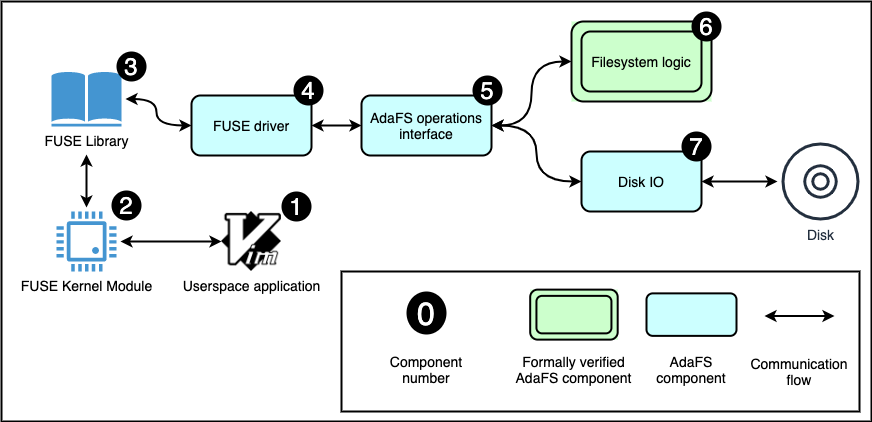
\includegraphics[scale=0.56]{design-overview.png}
  \caption{AdaFS design overview.}
  \label{fig:design overview}
\end{figure}


\subsection{Filesystem Organisation}
We next give an overview of the layout of the filesystem on disk, as well as the layout of various structures used in the filesystem.

A disk is formatted as an AdaFS filesystem using the \textit{mkfs} executable.
The resulting disk layout is shown in \autoref{fig:adafs disk layout}.
The disk is divided into blocks of 1024 bytes, similarly to MINIX.
Blocks are collected in zones, which can be of size $2^n$ blocks.
This abstraction of blocks into zones can make it possible to allocate multiple blocks at once.

\begin{figure}[tb]
  \centering
  
\includegraphics[scale=0.7]{disk-layout.png}
  \caption{AdaFS disk layout. (\textit{n} = number of inode bitmap blocks, \textit{m} = number of zone bitmap blocks, \textit{i} = number of inode blocks, \textit{s} = number of blocks on disk)}
  \label{fig:adafs disk layout}
\end{figure}

% \begin{figure}[tb]
%   \centering
%   \incfig{disk-layout}
%   \caption{AdaFS disk layout. (\textit{n} = number of inode bitmap blocks, \textit{m} = number of zone bitmap blocks, \textit{i} = number of inode blocks, \textit{s} = number of blocks on disk)}
%   \label{fig:adafs disk layout}
% \end{figure}

The disk begins with a boot block that would optionally contain executable code.
Then, it contains a superblock, and two bitmaps.
The bitmaps are used for inode and zone allocation, and can potentially span multiple blocks.
Next, there are a few blocks containing space for inodes, potentially with more than one inode per block.
Finally, the rest of the blocks contain user data.

The superblock is the second block on the disk, and contains information about the layout of the filesystem.
In particular, it contains the number of inodes and zones on disk, the number of inode and zone bitmap blocks, the number of the first data zone, the base-2 logarithm of the number of blocks per zone, the maximum file size, and the magic number.
The magic number used to identify a correctly formatted disk is $\text{CACA}_{16}$; MINIX uses the magic number $2468_{16}$, but AdaFS avoids using the same number, because a disk formatted by the AdaFS \textit{mkfs} utility is not necessarily equivalent to a disk formatted by the MINIX \textit{mkfs} utility.

The two bitmaps keep track of available inodes and zones, where the \textit{n}th bit of the inode or zone bitmap corresponds to the \textit{n}th inode or zone on disk, respectively.
If a bit in the inode bitmap is set to 1, that means the corresponding inode is allocated, and if it is set to 0, the inode is free.
This is the same for the zone bitmap, pertaining to zones.
One difference with MINIX is that, in MINIX, the first bit (bit zero) in the bitmaps must always be allocated, as the procedure that searches for a free inode or zone returns zero if no free inode/zone is found.
In Ada, indexing generally starts at 1, so all bits can be used -- as the first bit is bit one, this does not interfere with the allocation procedure.

The penultimate section of the disk contains inodes; the number of inodes is determined by the size of the disk.
The inodes have two representations: on-disk (\autoref{fig:inode on disk}) and in-memory (\autoref{fig:inode in memory}).
This allows the filesystem to make efficient use of disk space, while providing faster access to important values when the inode is loaded in memory.
There are 10 zones per inode: 7 direct zones (those that contain data), 1 single indirect zone (indicates a block that contains more direct zones), 1 double indirect zone (indicates a block that contains more single indirect zones), and 1 unused zone.
The unused zone is present for future use, potentially as a triple-indirect zone.

\begin{figure}[tb]
     \centering
     \begin{subfigure}[b]{0.45\textwidth}
         \centering
         
\includegraphics[scale=0.6]{inode-on-disk.png}
         \caption{On disk}
         \label{fig:inode on disk}
     \end{subfigure}
     \begin{subfigure}[b]{0.45\textwidth}
         \centering
         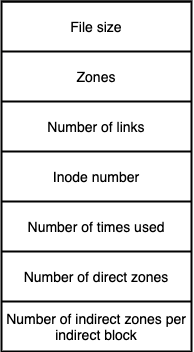
\includegraphics[scale=0.6]{inode-in-memory.png}
         \caption{In memory}
         \label{fig:inode in memory}
     \end{subfigure}
     \caption{Inode representations}
     \label{fig:inode representations}
\end{figure}


The final section spans the rest of the blocks on the disk, broken into zones, and is available to store user data.
It can contain file data, or directory entries.

There are also some in-memory structures for working with open files.
The filesystem keeps a process table in memory, which is indexed by process ID (PID), and keeps track of inode information for all processes using the filesystem.
One entry corresponds to one process, and contains the inode numbers for the root and working directories of the process, as well as the list of open file descriptors.
Each open file descriptor corresponds to an entry in the filesystem's \textit{filp} table, which is shared among all processes and contains all the file position.
The rationale for a shared file position table comes from MINIX, and is based on problems with the semantics of the \textit{fork} system call \cite{tanenbaum1997}.
An entry in the filp table contains the number of file descriptors using that entry, the inode number, and the file position for the inode.

Due to time constraints, a number of simplifications were made compared to MINIX.
In particular, only the features necessary for basic functionality of the system were implemented, and only file operations are supported (create, read, write, delete).
The filesystem does not cache any information, and there is no in-memory inode table; all data are written directly to disk.
Furthermore, the current implementation does not keep track of file mode, owner, group, or timestamps.
This results in a limited filesystem, which nonetheless completes its function as a proof-of-concept.

  \section{Implementation}
After discussing the high-level design of the filesystem, we explore the details of the implementation, with particular focus on elements that are specific to Ada/SPARK.
The filesystem is implemented using the Ada 2012 programming language.
Some parts of its parts are written in the SPARK 2014 language, which is a subset of Ada that removes features not amenable to formal verification, and defines new aspects to support modular, constructive, formal verification \cite{sparkRM}.
We use the AdaCore GNAT Community 2020 package\footnote{\url{https://www.adacore.com/community}}, which provides, among others, the compiler and prover tools.
For testing purposes, a FUSE driver is written in C, and the built executables are linked with libfuse 3.9.2\footnote{\url{https://github.com/libfuse/libfuse}}.
The GNAT Project Manager is used to facilitate compilation of source files in different languages and linking of other required libraries.

\subsection{Overview}
The implementation of AdaFS has \result{loc} lines of code: \result{loc-specification} lines for the specification, and \result{loc-implementation} for the implementation.
\autoref{tab:lines of code} shows the number of lines of code in the entire project, separated by component.
The component that defines filesystem logic has the most lines of code in the specification, as it also contains the formal verification code, which is placed in the specification files.
The disk IO component contains has the most lines of implementation code, as it takes care of the complexities of reading/writing data to disk.
The \textit{mkfs} utility does not contain any specification code, as it is not verified and it consists of a single main procedure (though it has nested procedures, those do not require a specification).

\begin{table}[tb]
  \centering
  \begin{tabular}{l | r | r}
    Component & Specification & Implementation \\
    \hline \hline
    Filesystem Logic & \result{loc-logic-specification} & \result{loc-logic-implementation} \\
    Disk IO & \result{loc-io-specification} & \result{loc-io-implementation} \\
    FUSE interaction & \result{loc-fuse-specification} & \result{loc-fuse-implementation} \\
    \textit{mkfs} utility & \result{loc-utility-specification} & \result{loc-utility-implementation}
  \end{tabular}
  \caption{Lines of code in AdaFS, separated by component.}
  \label{tab:lines of code}
\end{table}

\subsection{Language features}

\paragraph{Strong typing}
Ada is a strongly typed language, which helps the programmer distinguish between types that are logically different, even if their underlying representation is the same.
Furthermore, the compiler will automatically catch any bugs that would be caused by assigning a value of an incorrect type to a variable.
In order for a value to be assigned to a variable, two constraints must be satisfied: the value and variable must have the same type, and the value must satisfy all constraints on the variable (such as the range for an integral data type) \cite{barnes2014}.
Conversion between types is allowed, but only if it is explicit, and if the target type is an ancestor of the current type (for example, a positive integer may be converted to an integer, but not vice-versa).
An example of the use of types is the definition of a character buffer of arbitrary size, followed by the definitions of different block types including a constrained version of the buffer type, shown in \autoref{code:block type definitions}.

\begin{lstlisting}[float=tb,caption={Block type definitions}, label={code:block type definitions}, language=Ada]
type data_buf_t is array (Positive range <>) of Character;

type inode_block_t is array (1..block_size/on_disk'Size) of on_disk;
type zone_block_t is array (1..n_indirects_in_block) of Natural;
type dir_entry_block_t is array (1..block_size/direct'Size) of direct;
subtype data_block_t is data_buf_t (1..data_block_range'Last);
\end{lstlisting}

\paragraph{Controlled types}
Controlled types allow the programmer to specify precisely what happens when a variable of a given type is declared, or when it goes out of scope.
They are not permitted in SPARK, because the compiler inserts implicit calls to allow this functionality \cite{sparkRM}.
The initialization and destruction of variables of a controlled type is handled with custom \lstinline[language=Ada]{initialize} and \lstinline[language=Ada]{finalize} procedures for the type, thus the compiler needs to ensure these procedures are called in execution.
However, in AdaFS, controlled types are not used for any filesystem logic, and are only used with disk I/O to make sure that e.g. the variable containing the superblock is initialized properly with the type of I/O the filesystem uses.
Therefore, this was deemed acceptable for this prototype.

\paragraph{Lack of pointers}
The C codebase of MINIX makes extensive use of pointers to refer to inodes and other structures in memory, addresses on disk, etc.
Ada has access types, which are similar to pointers in some ways, but due to the complexity of verifying a program's behavior when it contains pointers, SPARK severely restricts the possibilities of using access types \cite{sparkRM}.
Thus, alternative methods must be used to provide similar functionality.

One way to solve this is with parameter modes.
Ada allows specifying the mode of each parameter in a procedure, which designates how the parameter will be used in execution.
If a parameter is of `in' mode, it is only read in the procedure, and is not modified -- this is the default mode.
If a parameter is of `out' mode, the value of the parameter before the call is irrelevant, as it will receive a value in the procedure.
Finally, if a parameter is of `in out' mode, it is both read and updated in the procedure.
This third mode provides functionality similar to a pointer.

However, SPARK requires that functions be purely functional; that is, they cannot have side effects, such as parameters with a mode of `out' or `in out'.
Here, two solutions are possible.
In some cases, it may be preferred to add the return value as an `out' parameter, and rewrite the function as a procedure.
In other cases, it is better for the function to return multiple values, which is possible with a record type.
An example is the function \lstinline[language=Ada]{parse_next} in \autoref{code:function returning record}, which returns two values, wrapped in the record type \lstinline[language=Ada]{parsed_res_t}.

\begin{lstlisting}[float=tb,caption={Parse function returning the parsed component and the new cursor position (ellipses denote code omitted for brevity)}, label={code:function returning record}, language=Ada]
subtype cursor_t is Natural range path'Range;

type parsed_res_t is record
  next : adafs.name_t;
  new_cursor : cursor_t;
end record;

function parse_next
  (path : adafs.path_t; cursor : cursor_t) return parsed_res_t
is
  ...
end parse_next;
\end{lstlisting}

\paragraph{Modularisation}
Ada supports modularisation in the form of packages, and forms a single translation unit, which can contain member entities such as subprograms, variables, and types.
Information hiding is done by defining members as private.
A package is separated into two parts, which are placed in separate files: the \textit{specification} (the public interface for the package), and the \textit{body} (the implementation).
The compiler always checks whether the package body matches the specification, and refuses to compile the code if this is not the case.
\autoref{code:inode specification and body} shows an excerpt of the specification and body of the \lstinline[language=Ada]{adafs.inode} package.

A package can also have child packages: for example, the \lstinline[language=Ada]{adafs.inode} package is a child of the \lstinline[language=Ada]{adafs} package.
A child package has access to all member entities defined in the specification of its parent(s), including private members.

\begin{lstlisting}[float=tb,caption={Excerpt from the adafs.inode package specification and body (ellipses denote code omitted for brevity)}, label={code:inode specification and body}, language=Ada]
-- adafs-inode.ads
package adafs.inode
  with SPARK_Mode
is
  ...
  function calc_num_inodes_for_blocks (nblocks : Natural) return Natural
    with ...;
end package adafs.inode

-- adafs-inode.adb
package body adafs.inode
  with SPARK_Mode
is
  function calc_num_inodes_for_blocks
    (nblocks : Natural) return Natural
  is
    inode_max : constant := 65535;
    i : Natural := nblocks/3;
  begin
    ...
    return i;
  end calc_num_inodes_for_blocks;
end adafs.inode;
\end{lstlisting}

It is also possible to create \textit{generics}.
Generics are somewhat similar to objects in the OOP paradigm, in that they can be instantiated with parameters.
However, an important difference is that instantiation can only occur in a declarative region.
Both subprograms and packages can be generic.
For example, \autoref{code:generic reading function} shows a generic function for reading data from a disk, and its instantiation.
A specification for a generic function \lstinline[language=Ada]{read_block} is defined in \textit{disk.ads}, accepting a numeric parameter between 0 and the disk size in blocks, and returning a result of the generic type \lstinline[language=Ada]{elem_t}.
In \textit{disk.adb}, the function is implemented.
If necessary, it first sets the disk file mode to read mode (\lstinline[language=Ada]{in_file}).
Then, it reads data of the generic type \lstinline[language=Ada]{elem_t} at the disk position corresponding to block number \lstinline[language=Ada]{num}, and returns these data.
The block-to-position conversion is handled by the \lstinline[language=Ada]{block2pos} function.
An example use of the generic function is in \textit{disk-inode.adb}, where the \lstinline[language=Ada]{read_block} function is instantiated with the data block type \lstinline[language=Ada]{data_block_t} (defined in another file to be an array of 1024 bytes).
The function instance is then used to read the data block \lstinline[language=Ada]{block_num}.

As Ada's \lstinline[language=Ada]{Stream_IO} always requires specifying the type to be read/written, using a generic function helps with code reuse.
\lstinline[language=Ada]{elem_t} is a generic type representing the type to be read or written; the concrete type is specified at instantiation.
The downside of generics is that they cannot be analyzed directly by SPARK, but must instead be verified from the context of instantiation (i.e., SPARK mode must be enabled in the package or subprogram that instantiates the generic) \cite{sparkRM}.

\begin{lstlisting}[float=tb,caption={Generic function for reading a block of type \textnormal{elem\_t}}, label={code:generic reading function}, language=Ada]
-- File: disk.ads
subtype block_num_t is Natural 0..disk_size_blocks;

generic
  type elem_t is private;
function read_block (num : block_num_t) return elem_t;

-- File: disk.adb
package SIO renames Ada.Streams.Stream_IO;
function read_block (num : block_num_t) return elem_t is
  result : elem_t;
begin
  if SIO.mode(disk) /= SIO.in_file then
    SIO.set_mode(disk, SIO.in_file);
  end if;

  SIO.set_index (disk, block2pos(num));
  elem_t'read (disk_access, result);
  return result;
end read_block;

-- File: disk-inode.adb
function read_chunk ... is
  function read_data_block is new read_block(data_block_t);
  data_block : data_block_t;
begin
  ...
  data_block := read_data_block(block_num);
  ...
end read_chunk;
\end{lstlisting}

\paragraph{Input \& output}
In AdaFS, we use a disk image file to represent the filesystem's disk.
Therefore, an appropriate way of reading and writing the file was needed.
Ada offers several types of input and output (IO), in the form of packages.
The simplest is \textit{Text\_IO}, which provides sequential file IO for human-readable text only.
The package \textit{Sequential\_IO} provides sequential access for heterogeneous data (data of varying types).
There are also two packages for random-access IO: \textit{Direct\_IO} and \textit{Stream\_IO}.
\textit{Direct\_IO} is used for files with homogeneous data (data of a single, uniform type), and \textit{Stream\_IO} is for heterogeneous data.

For this project, we required random-access IO, to allow the filesystem to read and write data at any position on the disk.
We also preferred heterogeneous IO, to be able to easily read and write data of varying types, such as different types of blocks (a data block, directory block, inode block, etc.).
Therefore, we opted for \textit{Stream\_IO}, as it best fulfilled our requirements.

\paragraph{Interfacing with other languages}
Ada has a mechanism to allow interfacing with other programming languages, such as Fortran, COBOL, or C.
This is done by replicating the types and subprogram signatures in Ada.
The Interfaces library package\footnote{\url{https://www.adaic.org/resources/add_content/standards/05aarm/html/AA-B-2.html}} provides types and subprograms for this purpose.
For example, for C, there are the Interfaces.C\footnote{\url{http://www.ada-auth.org/standards/12rm/html/RM-B-3.html}} and Interfaces.C.Strings\footnote{\url{http://www.ada-auth.org/standards/12rm/html/RM-B-3-1.html}} packages, which provide the types \lstinline[language=Ada]{chars_ptr} (mirroring \lstinline[language=C]{char*} in C), \lstinline[language=Ada]{int} (mirroring \lstinline[language=C]{int} in C), etc.
This allows \textit{exporting} subprograms from Ada, and calling them from a C program.
\autoref{code:interfacing c and ada} shows a specification of a subprogram that is exported to C by specifying the \lstinline[language=Ada]{Export} and \lstinline[language=Ada]{Convention} aspects (as well as an external name to use when calling the subprogram from C).
The subprogram is then declared as \lstinline[language=C]{extern} in C, and called from the C program's main function.
Since the main program is written in a language different from Ada, the initialization and finalization procedures (\lstinline[language=C]{adainit(void)} and \lstinline[language=C]{adafinal(void)}) must also be declared and called before and after any other Ada subprograms, respectively.
The GNAT Project Manager handles compiling and linking of files written in different languages.
Unfortunately, interfacing code is not amenable to formal verification.

\begin{lstlisting}[float=tb,caption={Interfacing code written in C and Ada. \textnormal{declarations.adb} is omitted for brevity, but is assumed to contain an implementation of the factorial function conforming to the specification.}, label={code:interfacing c and ada}, language=Ada, alsolanguage=C]
-- declarations.ads
with Interfaces.C;
package Declarations is
  function Factorial  (n : Interfaces.C.int) return Interfaces.C.int
    with Export => True,
         Convention => C,
         External_Name => "ada_factorial";
end Declarations;

-- main.c
#include <stdio.h>
extern void adainit (void);
extern void adafinal (void);
extern int ada_factorial(int n);

int main(int argc, const char *argv[]) {
  adainit();
  int n = 5;
  printf("%d\n", ada_factorial(n)); // 120
  adafinal();
}
\end{lstlisting}

\paragraph{FUSE \& the FUSE driver}
FUSE is a software interface that allows running filesystem code in userspace, with FUSE bridging the gap between the filesystem and the kernel.
This simplifies the development of filesystems, because access to the kernel and modification of kernel code is not necessary.
FUSE allows a filesystem to be developed iteratively; i.e., first it can be implemented and tested with FUSE, and later connected to a kernel if needed.

To implement a filesystem with FUSE, the code needs to be linked with the FUSE library (libfuse), and a driver must be written to specify the filesystem's handler functions for various operations.
As FUSE is written in C, the driver for AdaFS is currently also written in C, with a wrapper in Ada to convert values between C types and Ada types.
FUSE specifies a \lstinline[language=C]{struct} with pointers to functions that should be written by the programmer for the specific filesystem they are implemented.
The library also provides, among others, a function to fill file entries into a buffer, a \lstinline[language=C]{struct} to store open file information, and a function to get the context of the current operation (such as the PID requesting the operation).
\autoref{code:fuse open} shows an example from the driver, with an implementation of the open file operation.

FUSE also has support for multithreading and thus concurrent access.
However, this introduces a large amount of complexity, which is needed to handle concurrent access in a filesystem.
Therefore, we run FUSE in single thread mode (with the \textit{-s} flag on the command line), which ensures that there can only be one ongoing file operation at a given time.

\begin{lstlisting}[float=tb,caption={FUSE driver implementation of \textnormal{open}}, label={code:fuse open}, language=C]
#define FUSE_USE_VERSION 31
#include <fuse.h>
// Declare the external filesystem open function written in Ada
extern int ada_open(const char *path, pid_t pid);

// The driver's open function
int adafs_open(const char *path, struct fuse_file_info *finfo) {
  pid_t pid = fuse_get_context()->pid;
  int fd = ada_open(path, pid);
  finfo->fh = fd;
  return 0;
}

// Register the function with FUSE
static struct fuse_operations adafs_ops = {
  .open = adafs_open
};

int main(int argc, char **argv) {
  ...
  return fuse_main(argc, argv, &adafs_ops, NULL);
}
\end{lstlisting}

\paragraph{Formal verification}
Unfortunately, much of the code in its current form is not amenable to formal verification.
These are namely the parts involving file input and output, and functions that work with C types (i.e. the FUSE driver).
To mitigate this, we attempted to make use of an existing project containing FUSE bindings for Ada,\footnote{\url{https://github.com/medsec/ada-fuse}} but as the project has not been maintained since 2016, we were unable to compile it.

Nevertheless, large parts of filesystem logic are formally verifiable.
Therefore, the code base was split into two distinct packages: the \textit{adafs} package, which contains filesystem logic that is strictly in the SPARK language, and the \textit{disk} package, which contains unverifiable elements such as disk I/O.
The \textit{adafs} package does not include any specifics about the type of disk being used, as the \textit{disk} interface hides implementation details.
Thus, when needed, and when an alternative is found, the \textit{disk} package can simply be replaced with a verifiable implementation that exposes an identical interface.

For the parts that are formally verifiable, two types of contracts are available: functional and data contracts.
Functional contracts describe how a subprogram should function; that is, the pre- and post-conditions for a given subprogram.
They are written as boolean predicate logic expressions.
Pre-conditions are evaluated before entry into the subprogram, and post-conditions are evaluated after exit from the subprogram (and can therefore mention the subprogram's result).
SPARK can check these conditions at each call site to ensure that no subprogram call violates the conditions, and that the output(s) are shown to be conformant with the specification (the returned result for a function, and the \lstinline[language=Ada]{out} or \lstinline[language=Ada]{in out} parameters for a procedure).

The second type of contract available are data contracts.
SPARK conducts flow analysis, which models the flow of information during a subprogram's execution.
It checks for uninitialized variables, ineffective statements, and incorrect parameter modes.
It is possible to specify which global variables are read, written, or both read and written in the subprogram, using the \lstinline[language=Ada]{Global} aspect.
If no global variables are used, the value of the aspect is set to \lstinline[language=Ada]{null}.
It is also possible to specify data dependencies between a subprogram's inputs and outputs.

For example, \autoref{code:formal verification example} shows a function to get an entry from the process table, which specifies the functional and data contracts to be fulfilled for the function.
The \lstinline[language=Ada]{Global} aspect specifies that the function only depends on the value of the package variable \lstinline[language=Ada]{tab} for input.
The \lstinline[language=Ada]{Depends} aspect states that the result of the function only depends on the \lstinline[language=Ada]{tab} and \lstinline[language=Ada]{pid} variables (that is, the variable stated in the \lstinline[language=Ada]{Global} aspect, and the parameter of the function).
The post-condition states that the \lstinline[language=Ada]{is_null} component of the returned variant record will be set to True if there is no entry in \lstinline[language=Ada]{tab} for the provided PID; otherwise, the inode number of the PIDs working directory will be non-zero.
With the SPARK toolchain, we can verify that these constraints are all satisfied.

\begin{lstlisting}[float=tb,caption={Functional and data contracts}, label={code:formal verification example}, language=Ada]
function get_entry (pid : tab_range) return entry_t with
  Global => (input => tab),
  Depends => (get_entry'Result => (tab, pid)),
  Post => (if tab(pid).is_null
           then get_entry'Result.is_null
           else get_entry'Result.workdir > 0);
\end{lstlisting}

  \section{Results \& Evaluation}
We evaluate our implementation based on two metrics: \textit{correctness} and \textit{performance}.
Correctness relates to the functionality of the filesystem, i.e. to what degree the functionality of the implementation conforms to its specification.
Performance describes the speed and efficiency of the implementation.

\subsection{Correctness}
As stated earlier, the filesystem was split into two main parts: a filesystem logic part (the \textit{adafs} package), and an I/O part (the \textit{disk} package).
Because the logic part is easier to verify, it was the primary focus of formal verification for this project.
Currently, approximately 25\% of the filesystem is verified, and most of the unverified code is in the \textit{disk} package.
Since the FUSE driver is written in C, and in Ada with C types, it is also not verified.

We gave subprograms both functional and data contracts, as well as type definitions, according to their expected functionality.
Although this does not formally verify the functionality of the entire filesystem, it is a good starting point.
\autoref{code:prover summary} shows a summary of the conducted checks, and \autoref{code:prover output} shows some of the locations of various checks.

\begin{lstlisting}[float=tb,basicstyle=\tiny, caption={Prover summary (\textnormal{gnatprove}).}, label={code:prover summary}]
Summary of SPARK analysis
=========================

----------------------------------------------------------------------------------------------------------
SPARK Analysis results   Total        Flow   CodePeer                       Provers   Justified   Unproved
----------------------------------------------------------------------------------------------------------
Data Dependencies            5           5          .                             .           .          .
Flow Dependencies            4           4          .                             .           .          .
Initialization               1           1          .                             .           .          .
Non-Aliasing                 .           .          .                             .           .          .
Run-time Checks             17           .          .    17 (CVC4 89%, Trivial 11%)           .          .
Assertions                   2           .          .                      2 (CVC4)           .          .
Functional Contracts         6           .          .      6 (CVC4 92%, Trivial 8%)           .          .
LSP Verification             .           .          .                             .           .          .
Termination                  .           .          .                             .           .          .
Concurrency                  .           .          .                             .           .          .
----------------------------------------------------------------------------------------------------------
Total                       35    10 (29%)          .                      25 (71%)           .          .

max steps used for successful proof: 1

Analyzed 12 units
\end{lstlisting}

\begin{lstlisting}[float=tb,basicstyle=\tiny, caption={Excerpt from the prover output (\textnormal{gnatprove}).}, label={code:prover output}]
adafs-inode.adb:6:27: info: division check proved (CVC4: 1 VC in max 0.0 seconds and 1 step)
adafs-inode.adb:6:27: info: range check proved (CVC4: 1 VC in max 0.0 seconds and 1 step)
adafs-inode.adb:8:44: info: division check proved (CVC4: 1 VC in max 0.0 seconds and 1 step)
adafs-inode.adb:13:12: info: overflow check proved (CVC4: 1 VC in max 0.0 seconds and 1 step)
adafs-inode.adb:14:12: info: division check proved (CVC4: 1 VC in max 0.0 seconds and 1 step)
adafs-inode.adb:14:12: info: range check proved (CVC4: 1 VC in max 0.0 seconds and 1 step)
adafs-inode.adb:14:28: info: overflow check proved (CVC4: 1 VC in max 0.0 seconds and 1 step)
adafs-inode.ads:40:60: info: range check proved (CVC4: 1 VC in max 0.0 seconds and 1 step)
adafs-inode.ads:66:10: info: data dependencies proved
adafs-inode.ads:67:10: info: flow dependencies proved
adafs-inode.ads:69:18: info: postcondition proved (CVC4: 2 VC in max 0.0 seconds and 1 step)
adafs-proc.adb:6:14: info: discriminant check proved (CVC4: 2 VC in max 0.0 seconds and 1 step)
adafs-proc.adb:12:16: info: discriminant check proved (CVC4: 2 VC in max 0.0 seconds and 1 step)
adafs-proc.ads:26:05: info: data dependencies proved
adafs-filp.adb:18:30: info: loop invariant initialization proved (CVC4: 1 VC in max 0.0 seconds and 1 step)
adafs-filp.adb:18:30: info: loop invariant preservation proved (CVC4: 1 VC in max 0.0 seconds and 1 step)
adafs-filp.ads:28:13: info: postcondition proved (CVC4: 3 VC in max 0.0 seconds and 1 step)
adafs-filp.ads:32:28: info: initialization of "free_fd" proved
adafs-filp.ads:33:05: info: data dependencies proved
adafs-filp.ads:34:05: info: flow dependencies proved
adafs-filp.ads:35:13: info: postcondition proved (CVC4: 2 VC in max 0.0 seconds and 1 step)
\end{lstlisting}

The checks done by the prover can each be related directly to a Common Weakness Enumeration (CWE) number; these are shown in \autoref{tab:checks and cwe numbers} \cite{sparkUG}.

\begin{table}[tb]
  \centering
  \vspace{1em}
  \renewcommand{\arraystretch}{1.5}
  \begin{tabular}{| l | l |}
    \hline
    \textbf{Message} & \textbf{CWE number} \\ \hline
    divide by zero & 369 \\ \hline
    index check & 120 \\ \hline
    overflow check & 190 \\ \hline
    fp\_overflow check & 739 \\ \hline
    range check & 682 \\ \hline
    predicate check & 682 \\ \hline
    predicate check on default value & 682 \\ \hline
    null pointer dereference & 476 \\ \hline
    memory leak & 401 \\ \hline
    memory leak at end of scope & 401 \\ \hline
    discriminant check & 136 \\ \hline
    tag check & 136 \\ \hline
    use of an uninitialized variable & 457 \\ \hline
    precondition & 628 \\ \hline
    postcondition & 682 \\ \hline
  \end{tabular}
  \renewcommand{\arraystretch}{1}
  \vspace{1em}
  \caption{SPARK checks with their respective CWE numbers}
  \label{tab:checks and cwe numbers}
\end{table}

Due to Ada's type system, many of the checks do not take much effort to verify; in fact, all of the conducted checks were verified in one step.
The assurances provided by the prover are powerful, as they mean that e.g. overflow errors and range errors can \textit{never} happen at those locations.
In standard Ada, instructions are emitted to check that e.g. array accesses are within the bounds of the array.
However, with SPARK, such verifications can be conducted ahead of time (i.e. during compilation).
This means that the runtime checks done by Ada can be safely disabled, eliminating a number of machine instructions and thus improving the performance of the system.

The next step in verification would be to verify filesystem consistency, including consistency in the face of crashes.
This verification was not conducted in this paper, as the packages used for disk IO are not written in the SPARK subset of Ada, and are therefore not amenable to formal verification with SPARK.
However, it may be possible to implement a custom IO package that is written in SPARK, and could therefore be verified.
An alternative approach could be to verify the disk IO component using alternative methods, for example a modified version of Hoare Logic discussed in \autoref{sec:related work}, and this component would export several functions to the Ada filesystem.
A third option could be to implement a verified transactional log.

\subsection{Performance}
We conduct several tests to compare the performance of AdaFS with its C counterpart.
In particular, we would like to find out if the extra formal verification code results in decreased performance, as well as the effect that interfacing between C and Ada has on system performance.

\subsubsection{Microbenchmark comparison of Ada and C filesystem implementations}
We compare the performance of AdaFS with a C implementation of a FUSE-based MINIX 3 filesystem, fuse-mfs.\footnote{\url{https://github.com/redcap97/fuse-mfs}}
As AdaFS is not a complete filesystem, but only supports a small set of operations, it was not possible to use a standardised utility to test it.
Therefore, we created a microbenchmark in C that executes the relevant system calls and counts the number of CPU clock cycles necessary for each operation.
We compared some common filesystem operations, such as creating, writing, reading, and deleting files.
We used a virtual machine in VirtualBox 6.1.10 on a macOS host, running Debian 4.19.118, with FUSE version 3.4.1.
The host computer has an Intel Core i7-3615QM processor, with 4 physical cores and two threads per core, at 2.3 GHz.
The virtual machine is assigned 4 of these 8 virtual processors.
The disk images for the filesystem are stored on an SSD.

To calculate the number of CPU clock cycles an operation takes, we use a deterministic version of the ReaD Time Stamp Counter (RDTSC) instruction, RDTSCP, which is added as inline assembly in the C microbenchmark code.
The code to calculate elapsed clock cycles is shown in \autoref{code:rdtsc}.

\begin{lstlisting}[float=tb,caption={Calculating clock cycles.}, label={code:rdtsc}, language=C]
static __inline__ int64_t rdtsc_s(void) {
  unsigned a, d;
  asm volatile("cpuid" ::: "%rax", "%rbx", "%rcx", "%rdx");
  asm volatile("rdtsc" : "=a" (a), "=d" (d));
  return ((unsigned long)a) | (((unsigned long)d) << 32);
}

static __inline__ int64_t rdtsc_e(void) {
  unsigned a, d;
  asm volatile("rdtscp" : "=a" (a), "=d" (d));
  asm volatile("cpuid" ::: "%rax", "%rbx", "%rcx", "%rdx");
  return ((unsigned long)a) | (((unsigned long)d) << 32);
}
typedef int64_t cycle_t;

int main() {
  cycle_t cycles_before, cycles_after, cycles_per;
  cycles_before = rdtsc_s();
  // Call the test function here...
  cycles_after = rdtsc_e();
  cycles_per = cycles_after-cycles_before;
  printf("CPU cycles: %ld\n", cycles_per);
}
\end{lstlisting}

We choose RDTSCP instead of RDTSC because the CPU cannot reorder it relative to other instructions, as such reordering would cause noise in our results \cite{delorie2016}.
We set the \lstinline{isolcpus} kernel option at boot to isolate CPU 1, and then use the \lstinline{sched_affinity} function call to explicitly schedule each test on this CPU.
\autoref{code:schedule test} shows the code for this.

\begin{lstlisting}[float=tb,caption={Schedule a test on CPU 1.}, label={code:schedule test}, language=C]
#define _GNU_SOURCE
#include <sched.h>
void run_test(void) {
  // Schedule
  cpu_set_t the_cpu;
  int the_cpu_num = 1;
  CPU_ZERO(&the_cpu);
  CPU_SET(the_cpu_num, &the_cpu);
  if (sched_setaffinity(0, sizeof(the_cpu), &the_cpu) == -1) {
    perror("setaffinity failed");
  }

  // Run any tests below
  ...
}
\end{lstlisting}

We also assign interrupts to CPU 0 to avoid interference.
This ensures that no other processes are scheduled on the same CPU as our tests, i.e. that our results are as noiseless as possible.
We run FUSE in single-thread mode for both implementations of the filesystem.

We run the benchmark 30 times for each filesystem implementation; \autoref{tab:fs comparison} presents the median values for each implementation and operation.
It is apparent that AdaFS is significantly slower than fuse-mfs.
The largest difference is in the create operation, which is approximately 412.5 times slower.
The remove operation is around 2.5 times slower than that of fuse-mfs.
For other operations, the difference is not as drastic, though the Ada implementation is still around 10-20\% slower on average.

\begin{table}[tb]
  \begin{subtable}[t]{\textwidth}
    \centering
    \begin{tabular}{l r | r | r | r}
                      & \multicolumn{2}{c}{\underline{Create}}                                           & \multicolumn{2}{c}{\underline{Remove}} \\
       Implementation & Cycles                                 & Std. dev.                               & Cycles                   & Std. dev.                   \\
      \hline \hline
      AdaFS           & \result{adafs-create}                  & \result{adafs-create-stdev}             & \result{adafs-remove}    & \result{adafs-remove-stdev} \\
      fuse-mfs        & \result{fuse-mfs-create}               & \result{fuse-mfs-create-stdev}          & \result{fuse-mfs-remove} & \result{fuse-mfs-remove-stdev}
    \end{tabular}
    \caption{CPU cycles to create and remove files.}
    \label{tab:create remove files}
  \end{subtable}

  \bigskip

  \begin{subtable}[t]{\textwidth}
    \centering
    \small
    \begin{tabular}{l r | r | r | r | r | r | r | r}
                     & \multicolumn{2}{c}{\underline{Read 1 B}} & \multicolumn{2}{c}{\underline{Read 1 KB}} & \multicolumn{2}{c}{\underline{Read 10 KB}} & \multicolumn{2}{c}{\underline{Read 100 KB}} \\
      Implementation & Cycles                   & Std. dev.                      & Cycles                      & Std. dev.                         & Cycles                       & Std. dev.                          & Cycles                        & Std. dev.                        \\
      \hline \hline
      AdaFS          & \result{adafs-read-1}    & \result{adafs-read-1-stdev}    & \result{adafs-read-1024}    & \result{adafs-read-1024-stdev}    & \result{adafs-read-10240}    & \result{adafs-read-10240-stdev}    & \result{adafs-read-102400}    & \result{adafs-read-102400-stdev} \\
      fuse-mfs       & \result{fuse-mfs-read-1} & \result{fuse-mfs-read-1-stdev} & \result{fuse-mfs-read-1024} & \result{fuse-mfs-read-1024-stdev} & \result{fuse-mfs-read-10240} & \result{fuse-mfs-read-10240-stdev} & \result{fuse-mfs-read-102400} & \result{fuse-mfs-read-102400-stdev}
    \end{tabular}
    \caption{CPU cycles to read files of varying sizes.}
    \label{tab:read files}
  \end{subtable}

  \bigskip

  \begin{subtable}[t]{\textwidth}
    \centering
    \small
    \begin{tabular}{l r | r | r | r | r | r | r | r}
                     & \multicolumn{2}{c}{\underline{Write 1 B}} & \multicolumn{2}{c}{\underline{Write 1 KB}} & \multicolumn{2}{c}{\underline{Write 10 KB}} & \multicolumn{2}{c}{\underline{Write 100 KB}} \\
      Implementation & Cycles                                  & Std. dev.                                & Cycles                                    & Std. dev.                                   & Cycles                       & Std. dev.                          & Cycles                        & Std. dev.                        \\
      \hline \hline
      AdaFS          & \result{adafs-write-1}                   & \result{adafs-write-1-stdev}              & \result{adafs-write-1024}                  & \result{adafs-write-1024-stdev}              & \result{adafs-write-10240}    & \result{adafs-write-10240-stdev}    & \result{adafs-write-102400}    & \result{adafs-write-102400-stdev} \\
      fuse-mfs       & \result{fuse-mfs-write-1}                & \result{fuse-mfs-write-1-stdev}           & \result{fuse-mfs-write-1024}               & \result{fuse-mfs-write-1024-stdev}           & \result{fuse-mfs-write-10240} & \result{fuse-mfs-write-10240-stdev} & \result{fuse-mfs-write-102400} & \result{fuse-mfs-write-102400-stdev}
    \end{tabular}
    \caption{CPU cycles to write files of varying sizes.}
    \label{tab:write files}
  \end{subtable}
  \caption{Comparing filesystem operation performance in C (fuse-mfs) and Ada (AdaFS), showing the median and standard deviation across 30 observations.}
  \label{tab:fs comparison}
\end{table}

These differences in performance are mostly small enough that they are not generally noticeable in everyday life.
However, a create operation that takes 0.24 seconds (548615020 cycles at 2.3 GHz) may have a visible impact, and the other operations may also cause issues in applications where speed is critical.
Thus, it is important to find out why this slowdown happens, or eliminate factors that do not cause decreased performance.
It may not necessarily be due to the extra code needed for formal verification; AdaFS does not employ any optimisations or caching that MINIX 2 uses, and MINIX 3 is even more optimised for speed than MINIX 2.
For example, part of the \textit{create} operation is the creation of a new inode.
Among other things, MINIX keeps track of free inodes in a table in memory, which is flushed to disk at various points.
This makes looking up a free inode much faster, improving the performance of the \textit{create} operation.
Due to time constraints, AdaFS does not implement this table, and thus has to read it from the disk.
This is also the case with other similar mechanisms.

\subsubsection{The performance impact of formal verification code}
To determine if the verification code may play a role in the slowdown, we implemented two versions of a factorial function for numbers up to and including 20, in Ada.
We chose 20 because this is the highest possible number whose factorial is within the allowed range; Ada has support for larger numbers via various packages, but we opted not to use them so as not to introduce unnecessary overhead.
We use the same settings and pragmas as AdaFS.
One version includes a full formal specification, with data and functional contracts, and with type definitions.
The other version does not have any verification code whatsoever.
Both functions are exported to, and called from, C code; there is no parameter type conversion.

We run both implementations 500 times, counting the clock cycles.
The results (median and standard deviation) are shown in \autoref{tab:factorial comparison}.
From this, we see that the verified code actually seems to be faster.
However, the difference is only 4 clock cycles (1.2\%), so though verifying code with SPARK may allow the compiler to omit some instructions to check values and ranges, it is more probable that the difference is the result of some unknown interference.
For practical purposes, there does not seem to be a performance difference between code with formal verification annotations, and code without them.

\begin{table}[tb]
  \centering
  \begin{tabular}{l | r | r}
    Implementation & Cycles                         & Std. dev.                         \\
    \hline \hline
    Verified       & \result{factorial-verified}    & \result{factorial-verified-stdev} \\
    Unverified     & \result{factorial-nonverified} & \result{factorial-nonverified-stdev}
  \end{tabular}
  \caption{Factorial function comparison in Ada and C.}
  \label{tab:factorial comparison}
\end{table}

\subsubsection{The performance impact of C-to-Ada interfacing}
There is also another variable that must be accounted for: whether a function is called from C or from Ada.
The operations in AdaFS are called from C, with C types.
The C types passed into the function need to be converted to their corresponding Ada types, and then converted back when they are returned.
To see if some extra clock cycles might be used at this boundary, we implemented a function that takes an integer, multiplies it by two, and returns the result.
In C, this function is trivial; in Ada, the function converts the argument from the C integer type into Ada's Integer type, and then converts it back to a C integer when returning from the function.

We call both implementations from C code, and run them 500 times each, counting the clock cycles.
The median and standard deviation for both implementations are shown in \autoref{tab:interface comparison}.
We see that calling Ada code from C code adds 8 extra clock cycles (i.e. calling a function from Ada is 10\% slower).
This also probably varies depending on the number of parameter conversions that are necessary.

\begin{table}[tb]
  \centering
  \begin{tabular}{l | r | r}
    Implementation & Cycles & Std. dev. \\
    \hline \hline
    Ada & \result{intf-ada} & \result{intf-ada-stdev} \\
    C & \result{intf-c} & \result{intf-c-stdev}
  \end{tabular}
  \caption{The performance impact of interfacing with Ada.}
  \label{tab:interface comparison}
\end{table}

\subsubsection{Comparing the performance of random-access IO packages}
Another potential source of performance degradation could be the choice of IO package.
Ada offers two packages for random-access data IO: \textit{Stream\_IO} (heterogeneous data) and \textit{Direct\_IO} (homogeneous data).
In this project, we opted for the former, but the latter may offer better performance.
For example, because the implementation of \textit{Stream\_IO} might include some code to manipulate incoming or outgoing data into a suitable format.
To test whether this is the case, we implemented a function that opens a file, reads a record from the file, modifies the record, writes the modified record to the file, and closes the file.
We created two implementations, one with \textit{Direct\_IO}, and one with \textit{Stream\_IO}.
Both implementations exported functions to C, and both were called from C; this helped eliminate any potential clock cycle differences at the boundary between C code and Ada code.
We used the same setup as for the other tests (i.e. schedule the tests on an isolated CPU, and count clock cycles with RDTSC), and ran each implementation's function 500 times.
The results (median and standard deviation) are shown in table \autoref{tab:io implementation comparison}.

\begin{table}[tb]
  \centering
  \begin{tabular}{l | r | r}
    Implementation & Cycles & Std. dev. \\
    \hline \hline
    Stream IO & \result{stream-io} & \result{stream-io-stdev} \\
    Direct IO & \result{direct-io} & \result{direct-io-stdev}
  \end{tabular}
  \caption{Random-access IO implementation comparison in Ada.}
  \label{tab:io implementation comparison}
\end{table}

We can see that \textit{Stream IO} is actually faster than Direct IO, taking around 25\% fewer clock cycles for the same operations.
One reason might be because Direct IO could have some checks in place to verify that the data is indeed homogeneous.
The difference in clock cycles could also be the result of switching between reading and writing modes.
\textit{Stream IO} has a dedicated function to set the mode of the file, which may be optimised in some way, while with \textit{Direct IO}, the file has to be closed and reopened with the new mode.
Therefore, for the purposes of AdaFS where switches between file modes are common, \textit{Stream IO} seems more performant.
It could also be worthwhile to compare \textit{Stream IO} with one of the sequential IO packages, but as using only sequential reads and writes would require a different filesystem design or some levels of abstraction, it is not covered in this paper.

\subsubsection{Summary of performance evaluation}
Overall, there is quite a large difference between AdaFS and the C implementation of MINIX 3, with AdaFS being around 10-20\% slower on average, and the create operation being 412.5 times slower.
From follow-up testing, we found that interfacing between C and Ada adds 8 extra clock cycles, and that adding formal verification code to implementation code does not seem to impact performance.
We also compared two random-access IO packages, and found that using a homogeneous IO package does not seem to offer performance advantages over the heterogeneous IO package that we are currently using.
In summary, the performance difference we observe between AdaFS and its C counterpart is probably either due to optimisation differences, or due to some other variable that we have not tested.

  \section{Related Work} \label{sec:related work}
Having presented our design and implementation, we relate it to the existing body of work.
Other research has mainly focused on two areas: tools or frameworks for writing reliable filesystem code, and development of reliable filesystems themselves.

\subsection{Tools \& Frameworks}\label{subsec:tools frameworks}
Fryer et al. found that filesystem bugs that severely corrupt metadata are common, and that solutions to the necessary recovery procedures were unsatisfactory.
Therefore, they developed Recon, a system to protect filesystem metadata from arbitrary implementation bugs \cite{fryer2012}.
Recon sits between the filesystem and the block layer, and checks consistency invariants at commit points before allowing writes to disk.
Thus, failures that would be silent become detectable violations of these invariants.
Consistency invariants are declarative statements that must be satisfied before data is committed to disk, otherwise the filesystem may become corrupted.
The authors use the consistency rules used by a file system checker (\textit{e2fsck} in their implementation) to derive the invariants.
Consequently, the system can detect random corruption at runtime as effectively as a filesystem checker.
In essence, Recon can conduct online checks similar to those conducted by offline filesystem checkers (e.g. \textit{fsck}).
The disadvantage is that Recon is limited only to errors detectable by filesystem checkers, and it does not allow the programmer to specify which conditions should be checked.
Nevertheless, it is a general-purpose tool, and functions identically regardless of the implementation of various layers.

Another tool is COGENT, a new, restricted language developed by Amani et al. \cite{amani2016}, as an approach to writing and formally verifying high-assurance filesystem code.
It was designed to bridge the gap between the formal specification of a program and its low-level implementation, and to allow programmers that do not have a background in formal verification to provably avoid common errors.
Many of the characteristics required to guarantee the absence of common filesystem implementation errors were encoded in the language, which is strongly typed, type safe, and uses a linear type system (meaning that every variable must be used exactly once).
The compiler for the language generates C code and translation correctness proofs, enforces memory safety, and forbids undefined behavior in C code (such as null pointer dereferences or buffer overflows).
In evaluation, they found that code generated from COGENT has throughput that is almost identical to a C implementation, albeit with slightly higher CPU usage.
Though developing a language that has the necessary constraints encoded in its syntax and semantics may be a useful approach, the downside is that COGENT is very domain-specific.
This means that programmers would need to first learn the language, which may be more difficult given that it is a purely functional language whose type system is not very common, and people developing systems code are arguably more used to working with imperative languages.
However, it is important to note that the authors state that this was not a major barrier.

In 2016, Sigurbjarnarson et al. presented Yggdrasil, a toolkit which uses a push-button approach to formal verification \cite{sigurbjarnarson2016}.
Yggdrasil does not require manual annotations or proofs, and aids programmers by producing counterexamples for failed verification constraints.
To achieve this, the authors used \textit{crash refinement}, i.e. that the set of all disk states reachable in the implementation must be a subset of those allowed in the specification.
Push-button verification means that Yggdrasil asks the programmer to enter the specification of the expected behavior, the implementation, and any consistency invariants for the state of the filesystem image, and it then checks if the implementation meets the specification while satisfying the invariants.
All three inputs are written in the same language (a subset of Python), and Yggdrasil generates C code, which is compiled to an executable filesystem and can be mounted using the FUSE library.
The advantage is that proof is fully automatic, and does not require any special annotations in the code.
There is, however, the question of whether a high-level language such as Python provides access to all low-level functionality that a filesystem programmer may need, without importing modules (as it is unclear how imports are handled, and whether they are allowed).

Argosy is a framework to allow machine-checked verification of storage systems, and introduces recovery refinement, which is a set of conditions that guarantee that an implementation of an interface with a recovery procedure is correct \cite{chajed2019}.
Recovery refinement ensures correctness for anything using the specification, and can compose with other refinements to prove that an entire system is correct.
Its semantics are formulated in Kleene algebra.
The system implements Crash Hoare logic, which was introduced by and used in FSCQ, to prove recovery refinement.
Therefore, the authors produce a verified transactional disk API for unreliable disks.
Similarly to FSCQ, the code is verified using the Coq proof assistant, and produces Haskell code.

\subsection{Filesystems}
In 2014, Schellhorn et al. presented their work on a verified Flash filesystem \cite{schellhorn2014}.
Since Flash memory can only be written sequentially, and data in Flash memory cannot be overwritten in place (i.e. space can only be reused by erasing entire blocks), a special Flash file system must be used that is designed to work with Flash memory.
Flashix, the verified Flash filesystem they developed, is based on UBIFS.
They refined the high-level POSIX system interface using a Virtual Filesystem Switch (VFS) that maps POSIX operations to one or more Abstract File System (AFS) operations; the AFS is a model that captures the functional behavior of a specific filesystem \cite{ernst2012}.
The reason for this separation is that specific filesystems do not implement generic functionality, but instead satisfy an internal interface.
To provide safety for crashes, power cuts, and other such events, they used a transactional journal providing atomic writes \cite{ernst2015}.
They verified the code using the KIV interactive theorem prover, whose specification language is based on Abstract State Machines and Abstract State Machine refinement.
They then used tools to generate a Scala implementation, which could be mounted using the FUSE library and executed on the Java Virtual Machine.

FSCQ was the first file system that has a machine-checkable proof (as opposed to an interactive proof) that its specification and implementation match, and whose specification included crashes \cite{chen2015specifying}.
Chen et al. found that to achieve their design goals of atomic system calls, preventing real bugs, enabling proof automation, and allowing modularity, an extended variant of Hoare logic worked best \cite{chen2015using}.
Accordingly, they developed Crash Hoare logic, which allows programmers to write a specification of the behavior of a storage system in the face of a crash, and to prove them correct (i.e. if a computer crashes, the storage system will reboot into a state consistent with its specification).
This extension of Hoare logic takes into account the fact that during a crash, a procedure may stop at any point, and that recovery procedures may run.
The filesystem uses FscqLog, a write-ahead log also certified with Crash Hoare logic, which provides atomic transactions on top of asynchronous disk writes.
FSCQ was developed with the same features as the educational xv6 filesystem, which implements the Unix v6 filesystem with write-ahead logging.
The implementation used the Coq proof assistant, and generated Haskell code, which could be mounted with the FUSE library and a Haskell driver.
Based on FSCQ, DFSCQ (Deferred-write FSCQ) was later written to provide a precise specification for \textit{fsync} and \textit{fdatasync} in the case of log-bypass writes \cite{chen2017}.
Deferring writing data to persistent storage allow filesystem to achieve high I/O performance, and DFSCQ's implementation would provide crash safety for these operations.
In building DFSCQ, the authors presented a tree-based approach to specifying filesystem behavior, and a metadata-prefix specification to specify behavior for crashes.
Compared to FSCQ, DFSCQ has several optimisations and provides a number of missing features.
The approach of Chen et al. means that even the complex semantics of crashes and recovery procedures can be captured and verified.
However, it also means that a programmer wishing to use this system needs to be familiar with Coq's programming language, which is functional and dependently typed; this may be difficult for developers used to C-style languages.
Also, the resulting implementation is in Haskell, which may introduce overhead not present in C implementations.

Sigurbjarnarson et al. used Yggdrasil, discussed in \autoref{subsec:tools frameworks}, to implement a journaling filesystem: Yxv6.
This filesystem is similar to xv6 and FSCQ, with some differences.
To ensure correct atomicity of some operations, it manages opened files that have been unlinked using a partition for orphan inodes.
Unlike FSCQ, it uses validation, not verification, when managing free inodes and blocks; therefore, allocation of blocks or inodes may fail even if there is enough space.
The authors also implemented a verified version of the \textit{cp} utility, Ycp, and a verified implementation of the Arrakis \cite{peter2014} persistent log (Ylog).

  \section{Conclusion}
This paper aims to explore ways of writing reliable software, in particular reliable filesystems.
``A computer program does what you tell it to do, not what you want it to do'' \cite{bloch1997}, thus we investigate methods to allow the programmer to specify what they want a filesystem to do, so that it performs accordingly with minimal or no maintenance effort.
We highlight Ada and its SPARK subset, a programming language that has seen great success in industries requiring high-reliability software such as aviation and space exploration, but which has not yet, to the best of our knowledge, been used for the development of a filesystem.
As a proof-of-concept, we develop AdaFS, a small filesystem with components that are formally verified to perform according to their specification.
Our evaluation results indicate that formal verification, as well as the switch from the traditional choice of C to Ada, probably does not have a major impact on performance.

The goal of this paper is not to criticise or dismiss C, nor to suggest Ada as the sole alternative.
It is rather to explore tools that have not seen much use yet in the domain of filesystems.
Writing good, reliable C code is possible; one only needs to look at the number of large, widely-used C projects to see this.
Nonetheless, we hope this paper demonstrates that Ada is equally suitable as a low-level systems development language, while boasting features that allow programmers to ensure that their code runs exactly as intended, such as functional and data contracts.
These features not only provide developers with compile-time guidance, but also allow tools to prove the correctness of a program, which is more difficult to do for code written in C.
Given that Ada was designed specifically for cases where reliability is the primary concern, it only seems natural that it would excel in those cases.

Future work still needs to be done in this area to produce a filesystem that is suitable for regular use.
Many crucial optimisations and caching mechanisms are missing, and would need to be implemented.
The I/O part of the filesystem would need to be formally verified, perhaps using a variant of the Crash Hoare logic developed for other projects discussed in \autoref{sec:related work} to include system crashes and consistency constraints in the specification.
It could also be possible to implement a transactional log to ensure consistency.
Furthermore, the filesystem could be integrated with e.g. a formally verified operating system kernel \cite{king2019}, instead of running in userspace.
This would provide a solid foundation for reliable system development.

  \printbibliography

\end{document}
